\chapter{Persistent Homology} 
\label{chapter3-homology}

This chapter includes the necessary theoretical background of persistent homology. The main references for this chapter are (\cite{carlsson_topology_2009}) and (\cite{zomorodian_computing_nodate}).

\section{Motivation}

First of all, there are four major advantages for using topological methods to analyze high-dimensional point clouds.

\begin{enumerate}
	\item Topology provides qualitative information which is required for data analysis.
	
	\item Metrics are not theoretically justified. Compared to straightforward geometric methods, Topology is less sensitive to the actual choice of metrics. 
	
	\item Studying geometric objects using Topology does not depend on the coordinates. 
	
	\item Functoriality. This is the most important advantage.
	
	\begin{defn}[Functoriality]
	
		For any topological space X, abelian group $A$, and integer $k\geq 0,$ there is assigned a group $H_k(X,A).$ For any $A$ and $k$, and any continuous map $f: X \to Y,$ there is an induced homomorphism $H_k(f,A): H_k(X,A) \to H_k(Y,A).$ Then \underline{functoriality} refers to the following conditions:
		\begin{itemize}
			\item  $H_k(f\circ g,A): H_k(f,A) \circ H_k(g,A)$
			\item  $H_k(Id_{X};A) = Id_{H_k(X,A)}.$
		\end{itemize}
	\end{defn}
	Functoriality addresses the ambiguities in statistical clustering methods -- in particular the arbitrariness of various threshold choices. We now illustrate how exactly functoriality could be used in questions related to clustering. 
	
	Let $X$ be the full data set and $X_1,X_2$ are the subsamples from the data set. If the set of clusterings $C(X_1), C(X_2), C(X_1 \cup X_2)$ correspond well, then we can conclude that the subsample clusterings correspond to clusterings in the full data set $X$. 
\end{enumerate}

\section{Homotopy} \label{sec:homotopy}

\begin{defn}[Homotopy]

	\underline{Homotopy} is a family of maps $f_t: X \to Y$ where $t \in I$ such that $F: X\times I \to Y$ defined by $F(x,t) \mapsto f_t(x)$ is continuous.
	
	Two maps $f_0, f_1$ are \underline{homotopic} if there exists a homotopy $f_t$ between $f_0$ and $f_1$.  
\end{defn}

% A special case of homotopy is the deformation retraction. 

% \begin{defn}[Deformation retraction]
% 	A \underline{deformation retraction} of $X$ onto a subspace $A$ is a homotopy from the identity map of $X$ to a retraction of $X$ onto $A$, $r: X\to X$ such that $r(X) = A$ and $r|_A = \mathbbm{1}$ (or equivalently, retraction is the map $r: X\to X, r^2 =r$). 
% \end{defn}

% Retraction is the topological analog of projection. To visualize this analogy, we give an example of how some deformation retractions arise from the mapping cylinder.

% \begin{defn}
% 	For a map $f: X\to Y$, the \textit{mapping cylinder} $M_f$ is the quotient space of the disjoint union $(X \times I) \sqcup Y$.
% \end{defn}

\begin{defn}[Homotopy equivalence]

A map $f:X \to Y$ is a \underline{homotopy equivalence} if there is a map $g: Y \to X$ such that 
\begin{itemize}
	\item $f\circ g$ is homotopic to the identity map on $Y$, and
	\item $g\circ f$ is homotopic to $f$.
\end{itemize}

Two spaces $X,Y$ are\textit{ homotopy equivalent} if there exists a homotopy equivalence $f: X \to Y. $
\end{defn}

\begin{thm}
	If $f$ and $g$ are homotopic, then $H_k(f,A) = H_k(g,A).$ 
	
	If $X$ and $Y$ are homotopy equivalent, then $H_k(X,A) \cong H_k(Y,A) $.
	
	Note that if two spaces are homotopy equivalent, then all their Betti numbers (defined in subsequent section) are equal.
\end{thm}
\begin{defn}[Topological space]
    Associated to a simplicial complex $(V, \triangle)$ is a topological space $|(V,\triangle)|$. $|(V,\triangle)|$ may be defined using a bijection $\phi : V \to \{1, 2, \dots,N\}$ as the subspace of $\mathbb{R}^N$ given by the union 
	$$\bigcup_{\sigma \in \triangle} c(\sigma),$$
	where $c(\sigma)$ is the convex hull of the set $\{e_{\phi(s)}\}_{s\in \sigma}$, where $e_i$ denotes the $i$-th standard basis vector.

	 We often use abstract simplicial complexes to approximate topological spaces. For simplicial complexes the homology can be computed using only the linear algebra of finitely generated $\mathbb{Z}$-modules. In particular, for simplicial complexes, homology is algorithmically computable.
\end{defn}	
	
\begin{defn}[Nerve]
	Let $X$ be a topological space, and let $\mathcal{U} = \{U_\alpha\}_{\alpha\in A}$ be any covering of $X$. 
	
	The \underline{nerve} of $\mathcal{U}$, denoted by $N(\mathcal{U})$, will be the abstract simplicial complex with vertex set $A$, and where a family $\{\alpha_0, \dots, \alpha_k\}$ spans a $k$-simplex if and only if $U_{\alpha_0}\cap U_{\alpha_1} \cap \cdots \cap U_{\alpha_k} \neq \emptyset.$
\end{defn}

One reason that this construction is very useful in the following ``Nerve Theorem." This theorem gives the criteria for $N(\mathcal{U})$ to be homotopy equivalent to the underlying topological space $X$.

\begin{thm}[Nerve Theorem]
Suppose that $X$ and $U$ are as above, and suppose that the covering consists of open sets and is numerable. Suppose further that for all $\emptyset \subseteq A,$ we have that $\bigcap_{s\in S} U_s$ is either contractible or empty. Then $N(\mathcal{U})$ is homotopy equivalent to $X$.
\end{thm}
The Nerve Theorem is very important in TDA since it provides a way to encode the topology of continuous spaces into abstract combinatorial structures that are more useful for designing computationally efficient data structures and algorithms.

\section{Simplicial Complexes}

\begin{defn}[Simplicial complex]

	An \underline{abstract simplicial complex} is a pair $(V, \triangle)$, where $V$ is a finite set, and $\triangle$ is a family of non-empty subsets of $V$ such that 
	$$\tau \in \triangle \text{ and }\sigma \subseteq \tau \implies \sigma \in \triangle.$$
	
	$\tau \in \triangle $ is face of $\triangle$. The dimension of a face $\tau$ is $|\tau| - 1.$
	
	(Intuition) A simplicial complex $\triangle$ in $\mathbb{R}^n$ is a collection of simplices in $\mathbb{R}^n$ such that
	\begin{enumerate}
	    \item Every face of a simplex of $\triangle$ is in $\triangle$.
	    \item The intersection of any two simplicies of $\triangle$ is a face of each. 
	\end{enumerate}
\end{defn}

\begin{defn}[Maximal Face]

A face $\tau$ is a \underline{maximal face} of $\triangle$ if there is no face $\sigma$ of $\triangle$ such that $\tau \subsetneq \sigma.$
\begin{itemize}
    \item 0-dimensional faces: vertices
    \item 1-dimensional faces: edges
    \item A simplicial complex of dimension $D \leq 1$ is a simple and loopless graph.
\end{itemize}
\end{defn}

\begin{defn}[k-skeleton]

    A simplicial complex $\triangle_0$ is a subcomplex of $\triangle$ if $\triangle_0 \subseteq \triangle$.
    
    For $k\geq -1$, the \underline{k-skeleton} $\triangle^{(k)}$ of $\triangle$ is the subcomplex of $\triangle$ obtained by removing all faces of dimension higher than $k$. 
\end{defn}

\begin{defn}[f-vector]

    For each $n \geq -1,$ let $f_n = f_n(\triangle)$ be the number of faces of $\triangle$ of dimension $n$.
    
    The f-vector of $\triangle$ is the vector $(f_{-1}, f_0, f_1, \dots, f_d)$ where $d$ is the dimension of $\triangle$. 
    
    \begin{eg}
    Suppose the family of sets 
    $$\emptyset, \{a\},\{b\},\{c\}, \{d\}, \{a,b\}, \{a,c\}, \{b,c\}, \{b,d\}, \{c,d\}, \{a,b,c\}$$ form a simplicial complex $E_1$. Then the f-vector of $E_1$ is $(1,4,5,1)$.
    \end{eg}
\end{defn}

\begin{defn}[Oriented complex]

(Intuition) An \underline{oriented simplex} is a simplex $\sigma$ together with an orientation of $\sigma$. If $\{a_0, a_1, \dots, a_p\}$ spans a $p$-complex $\sigma$, then we denote the oriented simplex with $[a_0, a_1, \dots, a_p]$.

(Formal) Let $\mathbb{F}$ be a commutative ring, $\triangle$ be a simplicial complex. For each $n \geq -1,$ we form a free $\mathbb{F}$-module $\Chain_n(\triangle; \mathbb{F})$ with a basis indexed by the $n$-dimensional faces of $\triangle$. For each n-dimensional face $a_0 a_1\cdots a_n$, we have a basis element $\vec{e}_{a_0,a_1,\cdots, a_n}$. 

We refer to the basis element $\vec{e}_{a_0,a_1,\cdots, a_n}$ as an \underline{oriented simplex}. The concept of an oriented simplex is analogous to the idea of a unit vector (which gives the direction and has unit length).
\end{defn}

\begin{defn}[Chain group of degree $n$]
    We refer to the free $\mathbb{F}$-module $\Chain_n(\triangle; \mathbb{F})$ in the previous definition as the chain group of degree $n$. The rank of  $\Chain_n(\triangle; \mathbb{F})$ is the $n$-th value $f_n(\triangle)$ in the f-vector of $\triangle$.

\begin{eg}
For $E_1 = \{\emptyset, \{a\},\{b\},\{c\}, \{d\}, \{a,b\}, \{a,c\}, \{b,c\}, \{b,d\}, \{c,d\}, \{a,b,c\}\}$, we have the following chain groups of degrees $-1,0,1,2$, respectively:
\begin{itemize}
    \item $\Chain_{-1}(E_1) = \{\lambda e_{\emptyset}: \lambda \in \mathbb{F}\} \cong \mathbb{F}.$
    \item $\Chain_{0}(E_1) = \{\lambda_{a} e_{a} + \lambda_{b} e_{b}  + \lambda_{c} e_{c} + \lambda_{d} e_{d}: \lambda_{a}, \lambda_{b}, \lambda_{c}, \lambda_{d} \in \mathbb{F}\} \cong \mathbb{F}^4.$
    \item $\Chain_{1}(E_1) = \{\lambda_{a b} e_{a,b} + \cdots  + \lambda_{c d} e_{c,d} : \lambda_{a b}, \dots,  \lambda_{c d} \in \mathbb{F}\} \cong \mathbb{F}^5.$
    \item $\Chain_{2}(E_1) = \{\lambda e_{a,b,c}: \lambda \in \mathbb{F}\} \cong \mathbb{F}.$
\end{itemize}
\end{eg}
\end{defn}

\begin{defn}[Simplicial chain complex]
The \underline{simplicial chain complex} of a simplicial comlex $\triangle$, denoted with $C(\triangle)$, is defined as:

\begin{tikzcd}[cells={nodes={minimum height=2em}}]
\cdots\arrow[r,"\partial_{n+2}"] & 
\Chain_{n+1}(\triangle) \arrow[r,"\partial_{n+1}"] & 
\Chain_{n}(\triangle) \arrow[r,"\partial_{n}"] & 
\Chain_{n-1}(\triangle) \arrow[r,"\partial_{n - 1}"] &
\cdots
\end{tikzcd}

\begin{eg}
The simplicial chain complex of $E_1$,  $C(E_1)$ is 

\begin{tikzcd}[cells={nodes={minimum height=2em}}]
0\arrow[r] & 
\Chain_{2}(E_1) \arrow[r,"\partial_{2}"] \arrow[d, "\cong"] & 
\Chain_{1}(E_1) \arrow[r,"\partial_{1}"] \arrow[d, "\cong"] & 
\Chain_{0}(E_1) \arrow[r,"\partial_{0}"] \arrow[d, "\cong"] &
\Chain_{-1}(E_1) \arrow[r] \arrow[d, "\cong"] &
0\\
0\arrow[r] & \mathbb{F} \arrow[r,"\partial_{2}"] & \mathbb{F}^5  \arrow[r,"\partial_{1}"] & \mathbb{F}^4 \arrow[r,"\partial_{0}"] &
\mathbb{F}  \arrow[r] &
0
\end{tikzcd}
Recall that $E_1$ has f-vector $(1,4,5,1)$.
\end{eg}
\end{defn}
\begin{prop}[The double boundary condition]
\label{double-boundary}
Boundary maps satisfy the double boundary condition, that is, $\partial_n \circ \partial_{n+1} = 0 \quad \forall n.$
\end{prop}

\begin{defn}[Simplicial homology of degree $k$]
\label{kth-homology-group}
    (Intuition) The simplicial homology gives an algebraic measure on the amount of cycles that are not the boundaries. 

    (Formal) Define he $\mathbb{F}$-module $Z_k(\triangle; \mathbb{F})$ of cycles and the $\FF$-module of he boundary group $B_k(\triangle;\FF)$ by the following formulas:
    \begin{itemize}
        \item $Z_k(\triangle; \mathbb{F}) = ker(\partial_k) = \{Z \in \Chain_k(\triangle; \FF): \partial_k(Z) = 0\}$ 
        \item $B_k(\triangle;\FF) = im(\partial_{k+1}) = \{Z \in \Chain_k(\triangle; \FF): \partial_{k+1}(x), \quad x \in \Chain_{k+1}(\triangle; \FF)\}$ 
    \end{itemize}
    
    By \ref{double-boundary}, $B_k(\triangle;\FF)$ is a submodule of $Z_k(\triangle;\FF)$, i.e., $B_k(\triangle;\FF)\subseteq Z_k(\triangle;\FF) \subseteq C_k(\triangle;\FF)$. 
    
    We define the \underline{simplicial homology in degree $k$ of $\triangle$} to be the quotient group
    \begin{align}
        \Hom_k(\triangle;\FF) &= ker(\partial_k) / im(\partial_{k+1})\\
        &= Z_k(\triangle;\FF) / B_k(\triangle;\FF)
    \end{align}
\end{defn}

\begin{defn}[$k$-th Betti number]
\label{kth-betti}
    The $k$-th Betti number of the simplicial complex $\triangle$ is
    \begin{align}
        \beta_k(\triangle;\FF) &\coloneqq \dim \Hom_k(\triangle;\FF) \\
        &= \dim ker(\partial_k) - \dim im(\partial_{k + 1}).
    \end{align}
    
    \begin{itemize}
        \item elements in $ker(\partial_k)$ are called $k$-cycles.
        \item elements in $im(\partial_k)$ are called $k$-boundaries.
        \item $k$-cycles that are not boundaries represent $k$-holes, which means that the $k$-th Betti number $\beta_k(\triangle; \FF)$ is the number of $k$-holes. 
    \end{itemize}
\end{defn} 

\begin{defn}[Homology class]
Each member of $\Hom_k(\triangle;\FF)$ is a \underline{homology class}. Each such member is an equivalent class under the relation $z\sim z^\prime \iff z -z^\prime \in B_k(\triangle;\FF)$. 

Let $[z]$ denote the homology class containing the cycle $z$. 
\end{defn}

\begin{defn}[Homology as ``holes"]
In certain well-behaved cases, homology can be interpreted as an algebraic measure on the amount of ``holes" in a simplicial complex $\triangle$.

Formally, given $X\subseteq \RR^n$, a ``hole" of $X$ is a bounded connected component of $\RR^n\ X$. For a given $k\geq 0,$ suppose the $(k+1)$-skeleton $\triangle^{(k+1)}$ of $\triangle$ has a geometric realization $X \subseteq \RR^n$. Then $\Hom_k(\triangle;\FF)$ is a free $\FF$-module of rank equal to the number of holes of $X$. 

Homology associates a vector space $H_k(X)$ to a topological space $X$ for each $k\in \NN$.
\begin{itemize}
    \item $H_0(X)$ is the number of path components in $X$.
    \item $H_1(X)$ is the number of holes in X.
    \item $H_2(X)$ is the number of voids in X.
\end{itemize}
\begin{rmk}
Note, however, that in the general metric spaces, the interpretation that homology measures the amount of ``holes" does not hold.
\end{rmk}
\end{defn}

\section{Persistent homology}

The main idea of \textit{persistence} is that instead of selecting a fixed value of the threshold $\epsilon$, we would like to obtain a useful summary of the homological information for all the different values of $\epsilon$ at once. As $\epsilon$ increases, we add simplicies to the complexes and detect which features ``persist."

The main advantages of persistent homology are threefold: 
\begin{enumerate}
    \item It is based on algebraic topology.
    \item It is computable via linear algebra.
    \item It is robust with regards to perturbations in the input data. 
\end{enumerate}

\begin{defn}[Filtered simplicial complex]
\label{filtered}
A subcomplex of $\triangle$ is a subset $\triangle^i \subseteq \triangle$ that is also a simplicial complex. 
Let $\triangle$ be a finite simplicial complex and let $\triangle^1 \subset \triangle^2 \subset \cdots \subset \triangle^m = \triangle$ be a finite sequence of nested subcomplexes of $\triangle$. The simplicial complex $\triangle$ with such a sequence of subcomplexes, $\emptyset \subseteq \triangle^1 \subseteq \triangle^2 \subseteq \cdots \subseteq \triangle^m = \triangle$, is called \underline{filtered simplicial complex}.

% A \underline{filtration} on a simplicial complex $X$ is a collection of subcomplexes $\{X(t) \ |\ t\in \RR\}$ of $X$ such that $X(t) \subset X(t')$ whenever $t\leq t'$. The filtration value of a simplex $\sigma \in \triangle$ is the smallest $i$ such that $\sigma \in \triangle^i$. 
\end{defn}

\begin{defn}[$p$-persistent $k$-th homology group]
Given a filtered complex, for the $i$-th subcomplex $\triangle^i$ we can compute the associated 
\begin{itemize}
    \item the boundary maps $\partial_k^i$ for all dimensions $k$.
    \item boundary matrices $M_k^i$ for all dimensions $k$.
    \item groups $C_k^i, Z_k^i$ (cycle group), $B_k^i$ (boundary group), and $H_k^i$ (homology group).
\end{itemize}
Then the \underline{$p$-persistent $k$-th homology group} $H_k^{i,p}$ of $\triangle^i$ is 
\begin{itemize}
    \item $H_k^{i,p} = Z_k^i / (B_k^{i+p}\cap Z_k^i)$
    \item (equivalently) $H_k{i,p} \cong Im(\eta_k^{i,p})$, where $\eta_k^{i,p}$ is a bijection $\eta_k^{i,p}: H_k^i \to H_k^{i+p}$ that maps a homology class into another homology class containing it.   
\end{itemize}
Note that this is simply the definition of homology group of degree $k$ in Definition \ref{kth-homology-group} with the additional notion of persistence.
\end{defn}

\begin{defn}[$p$-persistent $k$-th Betti number]
We now have the persistent version of \ref{kth-betti}:

The $p$-persistent $k$-th Betti number of $\triangle^i$ is $\beta_k{i p} = $ the rank of the free subgroup of $H_k^{i,p}$.
\end{defn}


\begin{defn}[Persistence complex]
A \underline{persistence complex} $\mathscr{C}$ is a family of chain complexes $\{C^i_*\}_{i\geq 0 }$ over $R$, together with chain map's $f^i: C^i_* \to C^{i+1}_*$, so that we have the following diagram:

\begin{tikzcd}[cells={nodes={minimum height=2em}}]
C^0_* \arrow[r,"f^0"] & 
C^1_* \arrow[r,"f^1"] & 
C^2_* \arrow[r,"f^2"] & 
\cdots
\end{tikzcd}

The filtered simplicial complex defined in \ref{filtered} with inclusion maps for the simplices then becomes a \underline{persistence complex}. To illustrate, below is a portion of a persistence complex with the the chain complexes expanded. 

\begin{tikzcd}[cells={nodes={minimum height=2em}}]
                    \arrow[d,"\partial_3"]&                    \arrow[d,"\partial_3"]&                     \arrow[d,"\partial_3"] \\
C^0_2\arrow[r,"f^0"]\arrow[d,"\partial_2"]& C^1_2\arrow[r,"f^1"]\arrow[d,"\partial_2"]& C^2_2\arrow[r,"f^2"]\arrow[d,"\partial_2"]& \cdots\\
C^0_1\arrow[r,"f^0"]\arrow[d,"\partial_1"]& C^1_1\arrow[r,"f^1"]\arrow[d,"\partial_1"]& C^2_1\arrow[r,"f^2"]\arrow[d,"\partial_1"]& \cdots\\
C^0_0\arrow[r,"f^0"] & C^1_0 \arrow[r,"f^1"] & C^2_0 \arrow[r,"f^2"]& \cdots
\end{tikzcd}
\end{defn}

\begin{defn}[Persistence modules]
A \underline{persistence module} $\mathscr{M}$ is a family of $R$-modules $M^i$, together with homomorphisms $\phi^i: M^i \to M^{i+1}$.
\end{defn}

\begin{thm}[Classification Theorem]
    For a finite persistence module $\mathscr{M}$ with coefficients in the field $F$, 
    \begin{equation}
        H_*(\mathscr{M}; F) \cong \underbrace{\bigoplus_i x^{t_i}F(x)}_\text{free module} \oplus  \underbrace{\left(\bigoplus_j x^{r_j}(F(x)/(x^{s_j}F[x]))\right)}_\text{torsion module}
    \end{equation}
    
    There exists a bijection between the set of free elements and the set of homology generators with birth at $t_i$ and persist for all future parameter values. 
    
    There exists a bijection between the set of torsion elements and the set of homology generators with birth at $r_j$ and death at $r_j + s_j$. 
    
    The classification theorem gives the fundamental characterization of persistence barcode.
\end{thm}

\begin{thm}[Barcode as the persistence analogue of Betti number]
The rank of $H_k^{i\to j}(\mathscr{C}; F)$ gives the number of intervals in the barcode of $H_k^{i\to j}(\mathscr{C}; F)$ spanning the parameter interval $[i,j]$. In particular, $H_*^{i\to j}(\mathscr{C}^i_*; F)$ gives the number of intervals that contain $i$.
\begin{rmk}
As with Betti number, the barcode for $H_k$ does not give the actual structure of the homology group, but just a continuously parameterized rank. The barcode is useful in that it can qualitatively filter out topological noise (since they are ``short-lived" features) and capture significant topological features (features that persist over increasing values of $\epsilon$).
\end{rmk}
\end{thm}


% \begin{defn}
% 	Let $\underline{C}$ be any category, and $\mathcal{P}$ a partially ordered set. We regard $\mathcal{P}$
% 	as a category $\underline{\mathcal{P}}$ in the usual way, i.e. with object set $\mathcal{P}$, and with a unique morphism	from $x$ to $y$ whenever $x \leq y$. Then by a $\mathcal{P}$-persistence object in $C$ we mean a functor
% 	$\phi : \mathcal{P} \to C$.
	
% 	 More concretely, it means a family $\{c_x\}{x\in \mathcal{P}} $of objects of $C$ together with morphisms $\phi: xy : cx \to cy$ whenever$ x \leq y$, such that $\phi_{yz} \circ \phi_{xy} = \phi_{xz}$ whenever $x \leq y \leq z$. Note that the $\mathcal{P}$-persistence objects in $C$ form a category in their own	right, where a morphism $F$ from $\phi$ to $\Phi$ is a natural transformation. Again, in
% 	more concrete terms, a morphism from a family $\{c_x, \phi_{xy}\}$ to a family $\{d_x, \Phi_{xy}\}$ is a family of morphisms $\{f_x\}$, with $f_x : c_x \to d_x$, and where the diagrams commute:
% 	\begin{figure}[H]
% 		\centering
% 		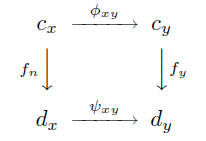
\includegraphics[width=0.3\linewidth]{figures/tda5-1.png}
% 		\label{fig:tda5-1}
% 	\end{figure}
% \end{defn}

% Although we do not have a classification theorem for $\mathbb{R}$-persistence abelian groups, which would then provide a summary of the behavior of the homology of all the complexes $\Cech(X,\epsilon)$, we do have a classification theorem for a subcategory of the category of $\mathbb{N}$-persistence $F$-vector spaces, where $F$ is a field. 

% From the $\mathbb{R}$-persistence simplicial complexes, we just need any partial order preserving map $\mathbb{N} \to \mathbb{R}$ to obtain an $\mathbb{N}-$persistence simplicial complex. Then we can use the classification theorem. 

% There are at least two useful ways to construct such maps. 

% The summary of the methodology is as follows:
% \begin{enumerate}
% 	\item Construct the $\mathbb{R}$-persistence simplicial complex using Cech, Vietoris-
% 	Rips, or witness methods. We will denote it by $\phi$.
% 	\item Select a partial order preserving map $f: \mathbb{N} \to \mathbb{R}$.
% 	\item Construct the associated N-persistence simplicial complex.
% 	\item Construct the associated N-persistence chain complex with coefficients
% 	in F. (It is evident from the finiteness hypotheses on X and
% 	the nature of the constructions that the associated N-persistence F-vector
% 	spaces are tame.)
% 	\item Compute the barcodes associated to the N-persistence F-vector spaces
% \end{enumerate}

\section{Commonly used complexes}

\begin{defn}[\v{C}ech complex]
	For any subset $V\subseteq X$ for which $X = \bigcup_{v\in V}B_\epsilon(v)$, one can construct the nerve of the covering $\{B_\epsilon(v)\}_{v\in V}$. This construction is referred to as the \underline{``\v{C}ech complex"} attached to $V$ and is denoted as $\Cech(V,\epsilon)$.
\end{defn}

\begin{thm}
Let $M$ be a compact Riemannian manifold. Then there is a positive number $e$ so that $\Cech(M, \epsilon)$ is homotopy equivalent to $M$ whenever $\epsilon \leq e$. Moreover, for every $ \epsilon \leq e$, there is a finite subset $V \subseteq M$ so that the subcomplex of $\Cech(V,\epsilon) \subseteq \Cech(M, \epsilon)$ is also homotopy equivalent to $M$.
\end{thm}

However, this construction is computationally expensive. A solution is to construct a simplicial complex which can be recovered solely from the edge information, which motivates the following construction known as the ``Vietoris-Rips complex." 

\begin{defn}[Vietoris-Rips complex]
	Let $X$ be a metric space with metric $d$. Then the  \underline{Vietoris-Rips complex} for $X$, attached to the parameter $\epsilon$, denoted by $VR(X,\epsilon)$, will be the simplicial complex whose vertex set is $X$, and where $\{x_0,\dots, x_k\}$ spans a $k$-simplex if and only if $d(x_i,x_j) \leq \epsilon$ for all $0\leq i,j\leq k.$
\end{defn}

\begin{prop}
	Comparing the \v{C}ech complex and the VR compelx:
	$$ \Cech(X,\epsilon) \subseteq VR (X,2\epsilon) \subseteq \Cech(X,2\epsilon).$$
\end{prop}

However, even the VR complex is computationally expensive. A solution, again, is to use the Voronoi decomposition which studies the subspaces of Euclidean space. 

\begin{thm}[Voronoi decomposition]
	Let $X$ be any metric space, and let $\mathcal{L}\subseteq X$ be a subset (called the set of \textit{landmark points}). Given $\lambda \in \mathcal{L}$, we define the \textit{Voronoi cell} associated to $\lambda, V_\lambda$, by
	$$V_\lambda = \{x\in X| d(x,\lambda) \leq d(x,\lambda^\prime)\} \forall \lambda^\prime \in \mathcal{L}.$$
\end{thm}


\begin{defn}[Delaunay complex]
	Similar to how we define the \v{C}ech complex above, we define the \underline{Delaunay complex} attached to $\mathcal{L}$ to be the nerve of this covering.
\end{defn}

However, for finite metric spaces, the Delaunay complex generically produces degenerate (i.e. discrete) complexes with no $1$-simplices. To solve this, we modify the definition to accommodate pairs of points which are ``almost" equidistant from a pair of landmark points. We thus have the definition below: 

\begin{defn}[Strong witness complex]
	Let X be any metric space, and suppose we are given a finite set $\mathcal{L}$ of points in $X$ (called the landmark set), and a parameter $\epsilon> 0$. For every point $x \in X$, we let $m_x$ denote the distance from this point to the set $\mathcal{L}$, i.e., the minimum distance from $x$ to any point in the landmark set.
	
	Then we define the \underline{strong witness complex} attached to this data to be the complex $W^s(X,\mathcal{L}, \epsilon)$ whose vertex set is $\mathcal{L}$, and where a collection $\{l_0, \dots, l_k\}$ spans a $k$-simplex if and only if there is a point $x \in X$ (the witness) so that $d(x, l_i)\leq m_x + \epsilon$ for all $i$. 
	
	We can also consider the version of this complex in which the $1$-simplices are identical to those of $W(X,\mathcal{L},\epsilon)$, but where the family $\{l_0, \dots, l_k\}$ spans a $k$-simplex if and only if all the pairs $(l_i, l_j)$ are $1$-simplices. We will denote this by $W^s_{VR}$.
\end{defn}

A modified version of the strong witness complex is also useful:

\begin{defn}[Weak witness complex]
	We construct the \underline{weak witness complex}, $W^w(X,\mathcal{L}, \epsilon)$, attached to the given data by declaring that a family $\Lambda = \{l_0, \dots, l_k\}$ spans a $k$-simplex if and only if $\Lambda$ and all its faces admit $\epsilon$ weak witnesses. 
	
	Similar to the definition for strong witness complex, we can also consider the version of the weak witness complex in which the $1$-simplices are identical to those of $W(X,\mathcal{L},\epsilon)$, but where the family $\{l_0, \dots, l_k\}$ spans a $k$-simplex if and only if all the pairs $(l_i, l_j)$ are $1$-simplices. We will denote this by $W^w_{VR}$.
\end{defn}